\section{實驗}
本研究將真實度模型放在 Apache Spark 叢集當中運行,並且實際應用在串流XML文件上面。因串流資料講求即時接收即時處理,所以難在短時間內做真實度驗證。所以此模型使用在串流資料的環境下可以解決這樣的問題。本研究利用XML文件產生器\cite{xmlgen}來產生XML文件,且每一個文件的大小皆不相同,實驗會使用客戶端程式隨機挑選不同大小的文件進行上傳至串流伺服器,再由伺服器分別做資料前處理以及真實度計分,並且產生報表。\\\par
因為XML通常用於資料交換,所以單一檔案不會到GB等級,所以串流XML文件在本研究的設定會是小容量且持續產生的檔案流。
\subsection{真實度模型之串流XML文件應用架構}
本研究設計並實作真實度模型在 Apache Spark 叢集當中。Apache Spark 作為真實度計分伺服器,將接收來自客戶端傳送過來的資料,客戶端會使用 socket 將每一份XML 文件上傳至伺服器端。在Apache Spark 是使用 Spark Streaming 當中的 Socket streaming 來進行接收。而在 Socket streaming 當中會將接收到的資料進行處理並且儲存,再由真實度模型進行計分,以下將針對系統當中的傳送端、處理模組以及真實度計分模組做介紹。\\\par

在資料傳送端,本研究自行實作Socket客戶端進行資料的上傳,每一個檔案會以字串的形式來做上傳,也就是說實際上客戶端發送的是持續產生的字串流,整體發送的時序圖如圖\ref{dataflow}所示:
\begin{figure}[H]
\centering
\graphicspath{{/Users/FUDA/Documents/masterThesis/image/}}
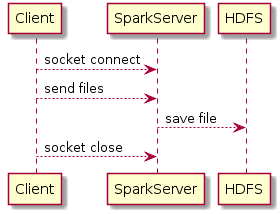
\includegraphics[scale=0.8]{dataflow.png}
\caption{資料接收與儲存流程}
\label{dataflow}
\end{figure}

在伺服器的處理模組使用的是Spark Streaming 來接收串流資料, 接收到串流資料的時候因資料是以字串流的方式發送的,所以資料處理模組會將字串流切分出每一個XML檔案,並且儲存至HDFS中。資料傳送處理流程如圖\ref{recv}所示:
\begin{figure}[H]
\centering
\graphicspath{{/Users/FUDA/Documents/masterThesis/image/}}
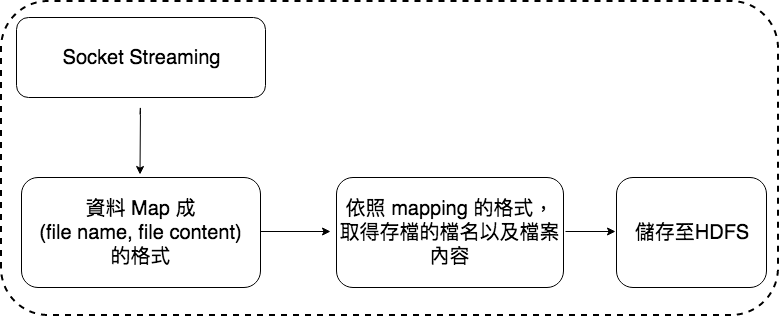
\includegraphics[scale=0.5]{recv.png}
\caption{資料傳輸處理模組}
\label{recv}
\end{figure}
在資料儲存的同時,真實度模型即開始從HDFS進行檔案的讀取,將傳送進來的XML文件與系統當中的基準文件做真實度計分,流程如圖\ref{process}所示:
\begin{figure}[H]
\centering
\graphicspath{{/Users/FUDA/Documents/masterThesis/image/}}
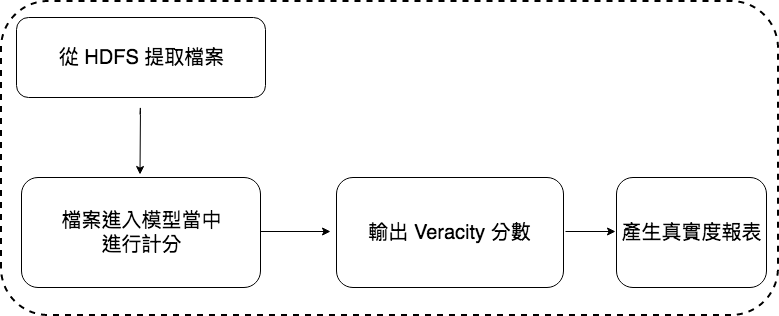
\includegraphics[scale=0.5]{process.png}
\caption{資料真實度計分模組}
\label{process}
\end{figure}

整體系統由傳送端、資料處理模組以及真實度模型計分模組所構成。利用串流做資料的上傳,從串流資料當中分割出每一個檔案來做儲存,並且使用真實度模型給予每一個檔案做真實度計分。完整系統架構如圖\ref{system}所示:
\begin{figure}[H]
\centering
\graphicspath{{/Users/FUDA/Documents/masterThesis/image/}}
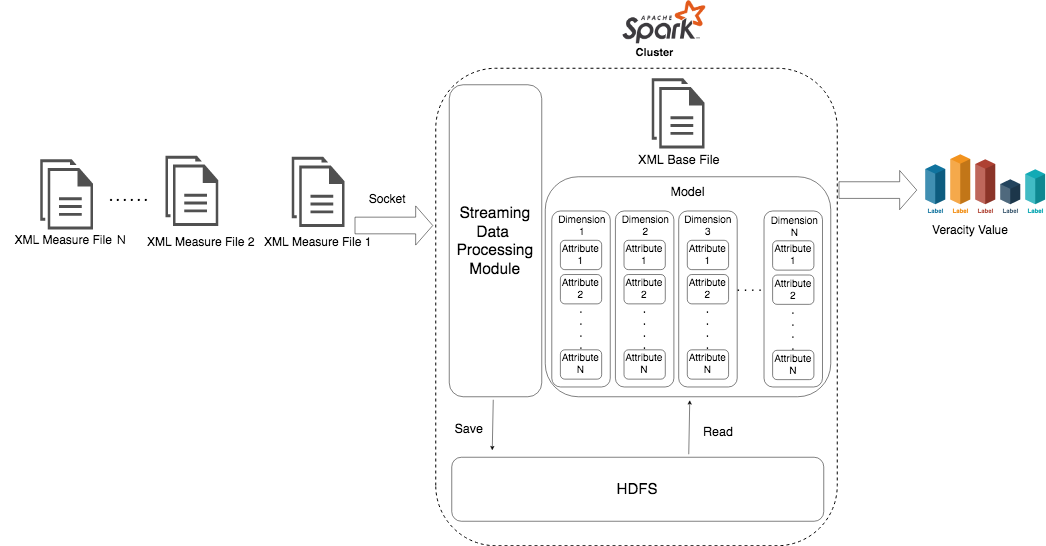
\includegraphics[scale=0.4]{VeracityArch.png}
\caption{系統架構圖}
\label{system}
\end{figure}
\newpage
\subsection{真實度模型之應用實例}
本研究設計之真實度模型API應用在前面所提到的串流XML文件上,藉由實驗,驗證真實度模型應用於串流XML文件的可行性。而由於真實度的計算方式可彈性由使用者自行設計,所以根據前面的抽象類別,在真實度模型的設計應用上,本實驗設計了兩個維度的真實度模型作為計算XML真實度的應用範例。\\\par
實驗設計的XML資料真實度應用範例具有兩個維度,分別是XML文件宣告以及XML文件結構。文件宣告的維度當中有文件編碼、文件版本以及是否為standalone等3個屬性,文件結構的維度當中有文件深度以及是否使用DTD或是Scheme 等2個屬性。圖\ref{veracitymodel}為設計的模型架構:
\begin{figure}[H]
\centering
\graphicspath{{/Users/FUDA/Documents/masterThesis/image/}}
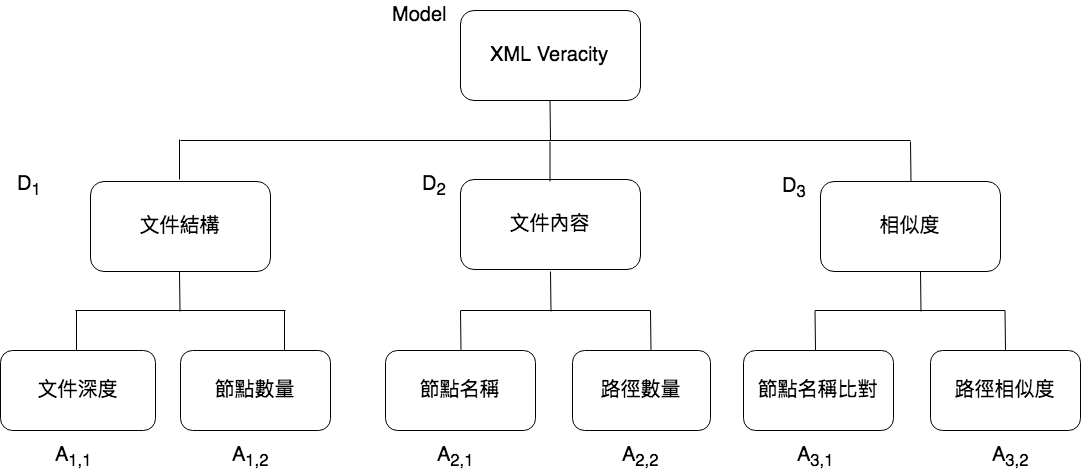
\includegraphics[scale=0.5]{xmlVeracity.png}
\caption{真實度模型}
\label{veracitymodel}
\end{figure}

這樣的架構可以對應到前面所提到的理論模型,在維度方面的定義$D_1$為XML文件宣告,$D_2$為XML文件結構:
$$
M=\{D_1,\ D_2\}\\
$$
在$D_1$維度下會有3個屬性$A_{1,1}$、$A_{1,2}$和$A_{1,3}$,$A_{1,1}$為XML文件編碼,$A_{1,2}$為XML版本,$A_{1,3}$為是否該文件為獨立存在:
$$
D_1=\{A_{1,1},\ A_{1,2},\ A_{1,3}\}\\
$$
而在$D_2$維度下會有三個屬性$A_{2,1}$以及$A_{2,2}$。而屬性$A_{2,1}$代表文件深度,$A_{2,2}$代表是否使用 DTD/Scheme:
$$
D_2=\{A_{2,1},\ A_{2,2}\}\\
$$
理論模型確立之後,即可以依照這樣的架構來實作模型,模型建立的演算法如圖\ref{createmodel}所示:
\begin{figure}[H]
\centering
\graphicspath{{/Users/FUDA/Documents/masterThesis/image/}}
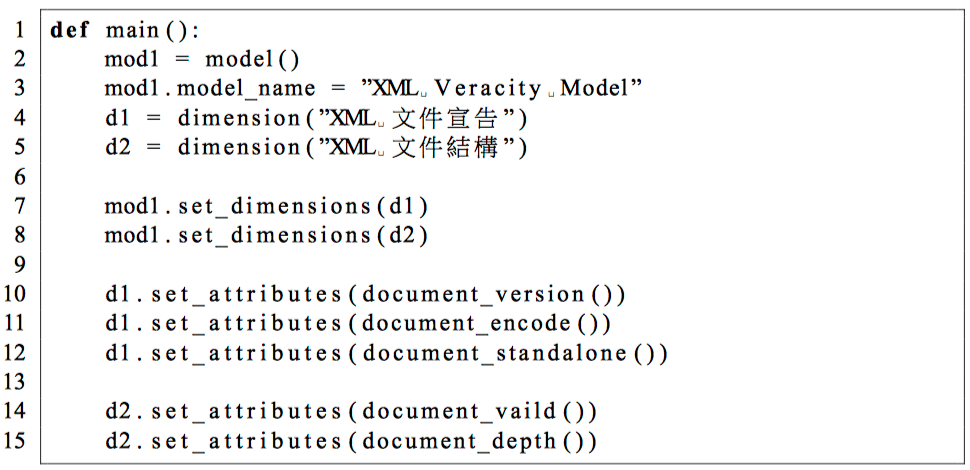
\includegraphics[scale=0.45]{createModel.png}
\caption{模型建立演算法}
\label{createmodel}
\end{figure}

接著需要設計每一個屬性都會有的一個計分方式(Quantification)。依文件宣告的維度來說,下面的兩個屬性:文件版本以及文件編碼,在文件版本來說,如果被量測文件與基準文件的版本不相同,那麼系統在分數的判定上會較為低分。如被測量文件與基準文件的版本是相同的,那系統的評分會是滿分。倘若在基準文件有做編碼宣告,但被量測文件並未做編碼宣告,那此項屬性的系統評分會是0分\\\par

而在文件編碼的部分,倘若被量測文件與基準文件採用相同編碼,則系統評分為滿分,如果不相同,但因為被量測文件還是有做編碼宣告,所以系統評分會是60分及格。如果基準文件有做編碼宣告而被量測文件沒有編碼宣告,此項屬性之系統評分則為0分。\\\par

再來是文件有無宣告standalone,standalone的宣告代表有沒有引用外部DTD,如果值為no,那就代表該文件的DTD是宣告在文件外部,如果值為yes,那代表DTD的宣告是在文件內部。如果被量測文件與基準文件的值同樣為yes或是no,那麼系統的評分會是滿分。若是被量測文件有宣告,但是裡面的值跟基準文件不同,則分數會稍微低一些。若是被量測文件無宣告standalone,屬性的系統評分為0分。\\\par

在文件結構的維度下會有兩個屬性:有無使用DTD/Scheme以及文件深度。在有無使用DTD/Scheme的部分,假設被量測文件與基準文件所使用的驗證方式相同,那麼系統計分會給高分,如果不相同,但是基於被量測文件仍然有使用驗證,所以系統會給及格分。假設被量測文件沒有使用任何驗證方式,那系統的屬性計分會給零分。\\\par
在文件深度的部分,實驗中以Dataguides\cite{oem}\cite{dataguides}\cite{oemweb}來進行計算,所謂的Dataguides是一種將XML的樹狀結構進行精簡化,來加速XML查詢以及節點走訪的速度,並且還可以保留各節點之間的關係。所以文件深度這一個屬性利用了Dataguides的特性來進行基準文件以及被量測文件的樹深度計算。如果兩棵樹深度相同。在系統計分上會為滿分,如果被量測文件的樹深度與基準文件相差2以內,則分數會照著比例增加。比方說基準文件深度為5,如果被量測文件的深度為6或是4,那分數的就為加20\%。如果深度的差距到達了2層以上,系統即認為被量測文件與基準文件的資訊差異過大,所以會以比例開始扣分。

\subsection{實驗環境}
實驗環境是使用建置在Openstack上面的虛擬機,共使用三個虛擬機。作業系統為Linux 發行版 Ubuntu 16.04 LTS,使用之CPU皆為8 核心,記憶體皆為16GB,表\ref{cluster}為機器的詳細規格。使用之Hadoop 版本為2.7,Spark版本為2.0。在HDFS中我們將每一個區塊的資料副本設置為3,軟體環境配置如表\ref{software}。
\begin{table}[H]
\begin{center}
\caption{叢集電腦規格}
\label{cluster}
\begin{tabular}{|p{3cm}<{\centering}|p{3cm}<{\centering}|p{3cm}<{\centering}|}
\hline
&Master 1台&Slave 2台\\
\hline
OS&Ubuntu 16.04 LTS&Ubuntu 16.04 LTS\\
\hline
CPU&Intel Core i7 8700@2.93GHz&Intel(R) Xeon(R) CPU E3-1230 v3 @ 3.30GHz\\
\hline
核心數&8&8\\
\hline
Memory&32 GB&12 GB\\
\hline
儲存空間&500 GB&1 TB\\
\hline
\end{tabular}
\end{center}
\end{table}

\begin{table}[H]
\caption{使用軟體版本}
\label{software}
\begin{center}
\begin{tabular}{|p{3cm}<{\centering}|p{3cm}<{\centering}|}
\hline
軟體名稱 & 版本號\\
\hline
Hadoop & 2.7版\\
\hline
Apache Spark &2.0版\\
\hline
Python & 3.6版\\
\hline
\end{tabular}
\end{center}
\end{table}

\newpage
\subsection{實驗設計}
實驗的設計主要分成三個部分,第一部分是自行設計的client端的傳送效率,在實驗中client端會隨機挑選數量不等的檔案進行上傳至server端,以此來測試每一個檔案的平均上傳時間。第二個部分為測試處理模組的效能,本實驗在測試從client接收資料到處理完畢存檔,每一個檔案的平均處理時間。最後一部分的實驗則是使用profiling的工具來測試本研究設計之真實度模型的效能。 \\\par %第三部分的則是測試真實度模型在計算大批次檔案的真實度計分的時候的平均處理時間。\\\par
第一部分的實驗將隨機從client挑選500個、700個以及900個檔案做發送,測試檔案的平均發送時間。第二部分的實驗將從client接收串流檔案,數量分別是500個、700個以及900個來做處理。並且將伺服器端設定成每3秒接收一次串流,來測試每一個微批次的處理時間。最後一部分為真實度模型實作在Apache Spark 中並且使用profiling的工具來測試效能。測試資料會從前次傳送的檔案中選擇檔案容量最大以及最小的檔案,藉由效能測試工具來檢視真實度模型的計算能力,並且從報表以及圖表中了解效能瓶頸。

\subsection{實驗結果}
在實驗結果方面,第一部分要看的是client端送效率,client端會從本地隨機挑選500個、700個以及900個檔案大小均不同的檔案,來看傳送速率。圖\ref{lab1}當中橫軸為每次傳送的檔案數量,縱軸為每一次傳送的平均時間,單位是秒。\\\par
\begin{figure}[H]
\centering
\graphicspath{{/Users/FUDA/Documents/masterThesis/image/}}
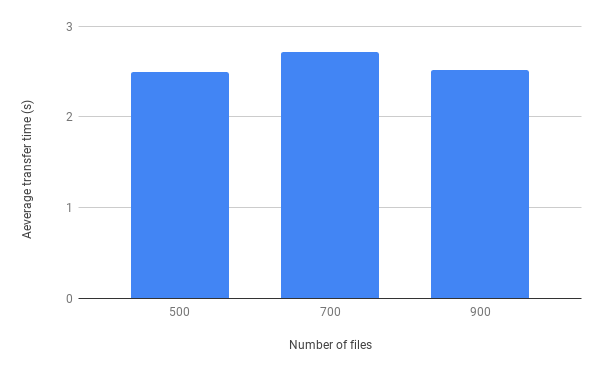
\includegraphics[scale=0.65]{lab1.png}
\caption{client傳送速率實驗}
\label{lab1}
\end{figure}
表\ref{lab1table}則是這次實驗的詳細數據。可以看到每一次的檔案傳送在時間上都是十分接近的,三次實驗的時間平均值約為2.57秒。\\\par
\begin{table}[H]
\caption{client傳送速率實驗詳細數據}
\label{lab1table}
\begin{center}
\begin{tabular}{|p{2cm}<{\centering}|p{2.7cm}<{\centering}|p{2.7cm}<{\centering}|p{2.7cm}<{\centering}|p{2.7cm}<{\centering}|}
\hline
檔案數量 & 平均傳送時間 & 檔案平均大小 & 最大傳送檔案 & 最小傳送檔案\\
\hline
500 & 2.49秒 & 28.57MB & 57.91 MB & 0.17 MB\\
\hline
700 & 2.71秒 & 28.05MB & 57.91MB & 0.14 MB\\
\hline
900 & 2.51秒 & 29.14MB& 58.09 MB & 0.14 MB\\
\hline
\end{tabular}
\end{center}
\end{table}
\newpage
第二部分的實驗則是server的處理模組在接收到串流資料的平均處理時間,這次的實驗會接收500個、700個以及900個檔案大小均不同的檔案,並且計算每一個檔案的平均處理時間。圖\ref{lab2}為三次實驗之統計數據,橫軸為檔案數量,縱軸為單一檔案平均處理時間。
\begin{figure}[H]
\centering
\graphicspath{{/Users/FUDA/Documents/masterThesis/image/}}
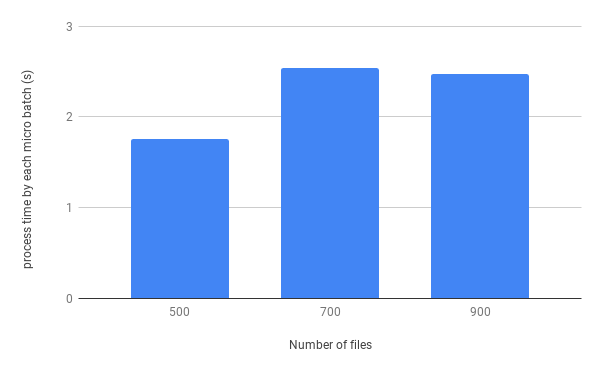
\includegraphics[scale=0.65]{lab2.png}
\caption{處理模組之處理速度實驗}
\label{lab2}
\end{figure}
表\ref{lab2table}為此次實驗之詳細數據,可以發現處理模組的處理速度平均值約在2.254秒左右,另外可以觀察到的是在檔案數量提升到了700與900的時候,處理速度上也提升到了單一檔案平均2.4秒以上。
\begin{table}[H]
\caption{server端處理模組處理速率實驗詳細數據}
\label{lab2table}
\begin{center}
\begin{tabular}{|p{3cm}<{\centering}|p{3cm}<{\centering}|}
\hline
檔案數量 & 單一檔案平均處理時間\\
\hline
500 & 1.754秒 \\
\hline
700 & 2.536秒 \\
\hline
900 & 2.472秒 \\
\hline
\end{tabular}
\end{center}
\end{table}

最後一部分的實驗為真實度模型實作在Apache Spark 中並且使用profiling的工具來測試效能。本次實驗使用的效能量測工具為cProfile\cite{prof},cProfile 為C語言實作的Python 效能量測工具,藉由這項工具可以量測出程式當中每一個函數的執行時間以及呼叫次數等相關資料。本次實驗挑選了五個檔案,詳細檔案數據如表\ref{500maxmin}、表\ref{700maxmin}以及表\ref{900maxmin}所示,這5個檔案分別會進行profiling的測試,以找出真實度模型的效能問題點。

%30 document_version
%45 document_encoding
% 70 document_standalone
% 93 document_valid
% 112 document_depth
\begin{table}[H]
\caption{傳送500個檔案當中的最大檔案以及最小檔案}
\label{500maxmin}
\begin{center}
\begin{tabular}{|p{3cm}<{\centering}|p{3cm}<{\centering}|}
\hline
檔案名稱 & 檔案大小\\
\hline
doc10.xml & 0.17 MB \\
\hline
doc5216.xml & 57.91 MB \\
\hline
\end{tabular}
\end{center}
\end{table}

\begin{table}[H]
\caption{傳送700個檔案當中的最大檔案以及最小檔案}
\label{700maxmin}
\begin{center}
\begin{tabular}{|p{3cm}<{\centering}|p{3cm}<{\centering}|}
\hline
檔案名稱 & 檔案大小\\
\hline
doc4.xml & 0.14 MB \\
\hline
doc5216.xml & 57.91 MB \\
\hline
\end{tabular}
\end{center}
\end{table}

\begin{table}[H]
\caption{傳送900個檔案當中的最大檔案以及最小檔案}
\label{900maxmin}
\begin{center}
\begin{tabular}{|p{3cm}<{\centering}|p{3cm}<{\centering}|}
\hline
檔案名稱 & 檔案大小\\
\hline
doc3.xml & 0.14 MB \\
\hline
doc5223.xml & 58.09 MB \\
\hline
\end{tabular}
\end{center}
\end{table}
首先先針對表\ref{500maxmin}的檔案進行profiling,並且將結果視覺化,如圖\ref{min500}和圖\ref{max500}所示。在doc10.xml的實驗當中,總計算時間為8.980 秒,最花費效能的是main:30的函數,消耗了29.23\%的時間。其次是main:93的函數,消耗了14.08\%的時間,詳細數據如表\ref{doc10pro}所示。而在doc5216xml的實驗當中總計算時間為49.719 秒,最花費效能的是main:93的函數,消耗了34.19\%的時間。其次是main:30的函數,消耗了16.36\%的時間,詳細數據如表\ref{doc52161pro}所示。

\begin{figure}[H]
\centering
\graphicspath{{/Users/FUDA/Documents/masterThesis/image/}}
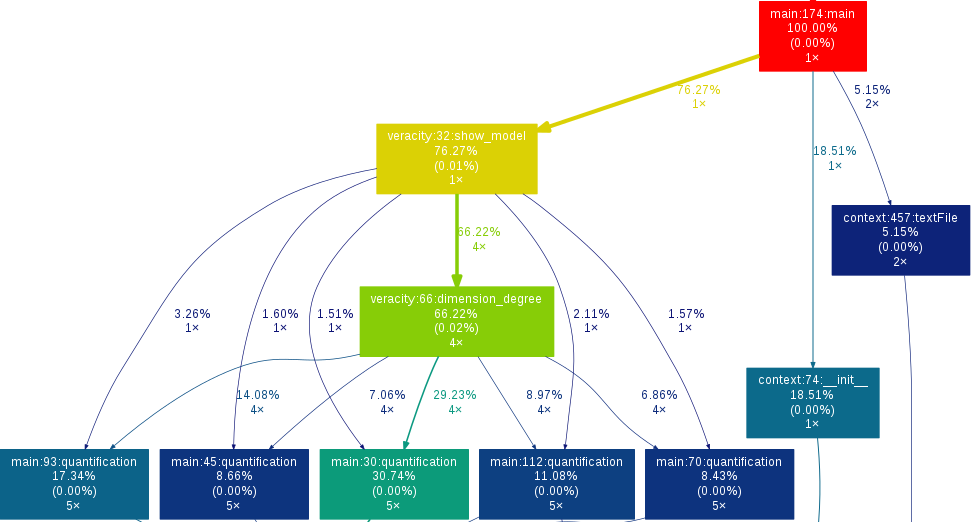
\includegraphics[scale=0.45]{min500.png}
\caption{doc10.xml profiling 效能分析}
\label{min500}
\end{figure}

\begin{figure}[H]
\centering
\graphicspath{{/Users/FUDA/Documents/masterThesis/image/}}
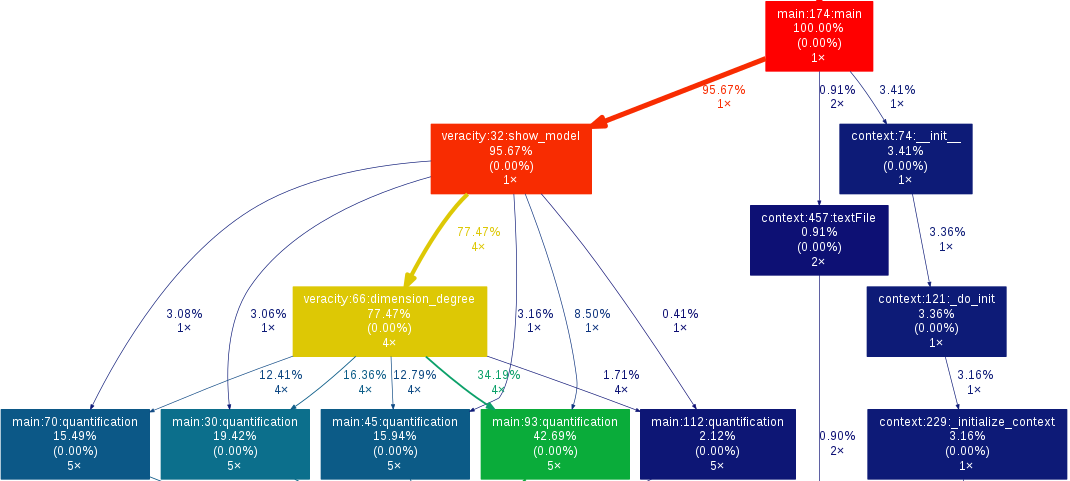
\includegraphics[scale=0.45]{max500.png}
\caption{doc5216.xml profiling 效能分析}
\label{max500}
\end{figure}

\begin{table}[H]
\caption{doc10.xml 計算效能}
\label{doc10pro}
\begin{center}
\begin{tabular}{|p{4cm}<{\centering}|p{3cm}<{\centering}|}
\hline
物件名稱 & 消耗效能 (\%)\\
\hline
document\_version & 30.74 \\
\hline
document\_encoding & 8.66 \\
\hline
document\_standalone & 8.43 \\
\hline
document\_valid & 17.34 \\
\hline
document\_depth & 11.08 \\
\hline
\end{tabular}
\end{center}
\end{table}

\begin{table}[H]
\caption{doc5216.xml 計算效能}
\label{doc52161pro}
\begin{center}
\begin{tabular}{|p{4cm}<{\centering}|p{3cm}<{\centering}|}
\hline
物件名稱 & 消耗效能 (\%)\\
\hline
document\_version & 19.42 \\
\hline
document\_encoding & 15.94 \\
\hline
document\_standalone & 15..49 \\
\hline
document\_valid & 42.69 \\
\hline
document\_depth & 2.12 \\
\hline
\end{tabular}
\end{center}
\end{table}
 第二個針對表\ref{700maxmin}做profiling的分析,profiling的視覺圖如圖\ref{min700}以及圖\ref{max700}所示。在doc4.xml 的profiling分析當中,總計算時間為9.412 秒,最消耗效能的是main:30的函數。而在doc5116.xml的總計算時間為50.856秒,當中最消耗效能的是main:93的函數。詳細實驗數據如表\ref{doc4pro}和表\ref{doc52162pro}所示。


\begin{figure}[H]
\centering
\graphicspath{{/Users/FUDA/Documents/masterThesis/image/}}
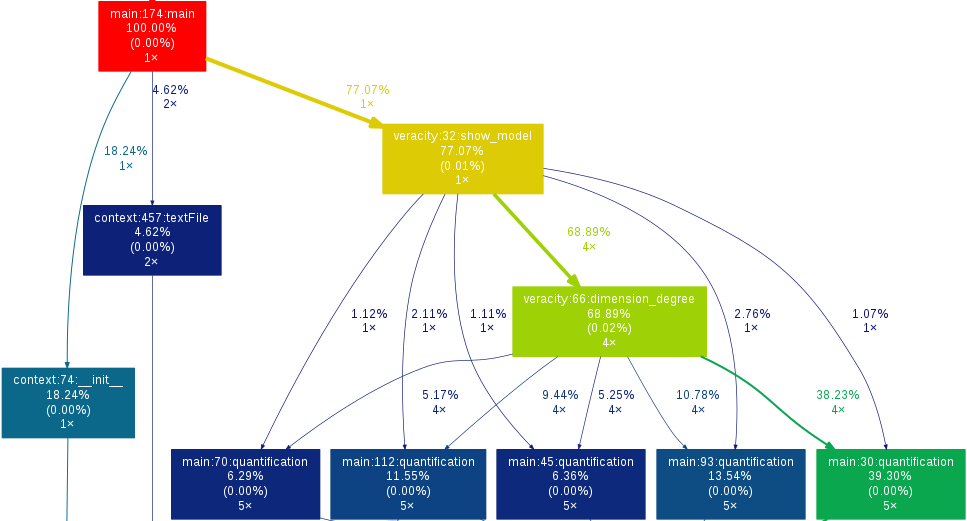
\includegraphics[scale=0.45]{min700.png}
\caption{doc4.xml profiling 效能分析}
\label{min700}
\end{figure}

\begin{figure}[H]
\centering
\graphicspath{{/Users/FUDA/Documents/masterThesis/image/}}
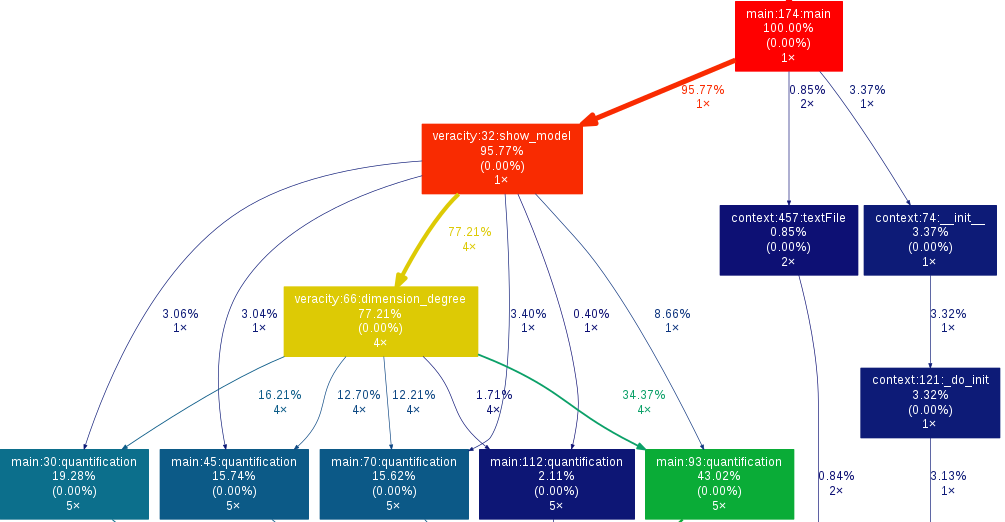
\includegraphics[scale=0.45]{max700.png}
\caption{doc5216.xml profiling 效能分析}
\label{max700}
\end{figure}


\begin{table}[H]
\caption{doc4.xml 計算效能}
\label{doc4pro}
\begin{center}
\begin{tabular}{|p{4cm}<{\centering}|p{3cm}<{\centering}|}
\hline
物件名稱 & 消耗效能 (\%)\\
\hline
document\_version & 39.30 \\
\hline
document\_encoding & 6.36 \\
\hline
document\_standalone & 6.29 \\
\hline
document\_valid & 13.54 \\
\hline
document\_depth & 11.55 \\
\hline
\end{tabular}
\end{center}
\end{table}

\begin{table}[H]
\caption{doc5216.xml 計算效能}
\label{doc52162pro}
\begin{center}
\begin{tabular}{|p{4cm}<{\centering}|p{3cm}<{\centering}|}
\hline
物件名稱 & 消耗效能 (\%)\\
\hline
document\_version & 19.42 \\
\hline
document\_encoding & 15.94 \\
\hline
document\_standalone & 15..49 \\
\hline
document\_valid & 42.69 \\
\hline
document\_depth & 2.12 \\
\hline
\end{tabular}
\end{center}
\end{table}
最後來看到表\ref{900maxmin}的profiling數據,視覺圖如圖\ref{min900}以及圖\ref{max900}所示。在doc3.xml的profiling當中,總計算時間為8.185秒,消耗最高的是main:30的函數。而在doc5223.xml的profiling當中,總計算時間為52.259秒,消耗最高的函數為main:93。詳細實驗數據如表\ref{doc3pro}與表\ref{doc5223pro}所示。
\begin{figure}[H]
\centering
\graphicspath{{/Users/FUDA/Documents/masterThesis/image/}}
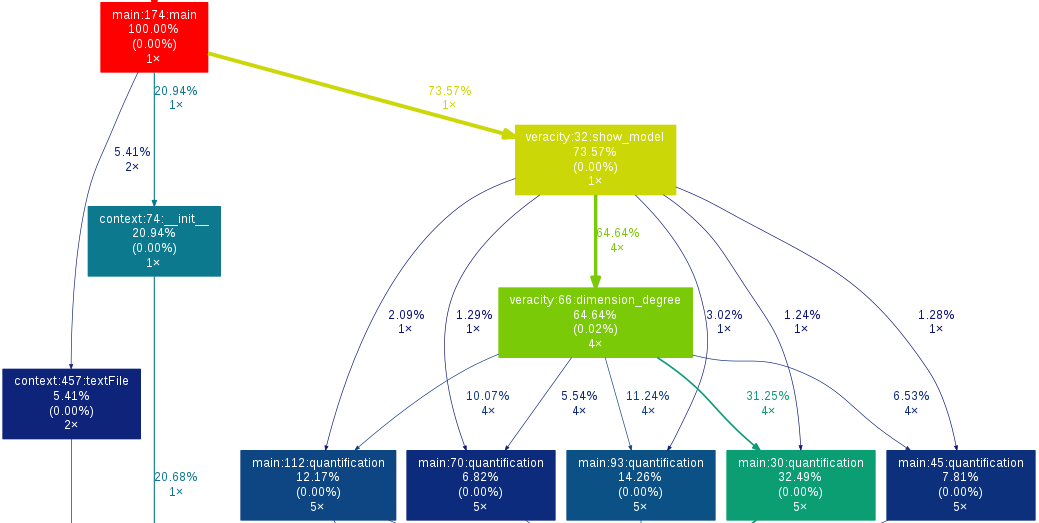
\includegraphics[scale=0.45]{min900.png}
\caption{doc3.xml profiling 效能分析}
\label{min900}
\end{figure}

\begin{figure}[H]
\centering
\graphicspath{{/Users/FUDA/Documents/masterThesis/image/}}
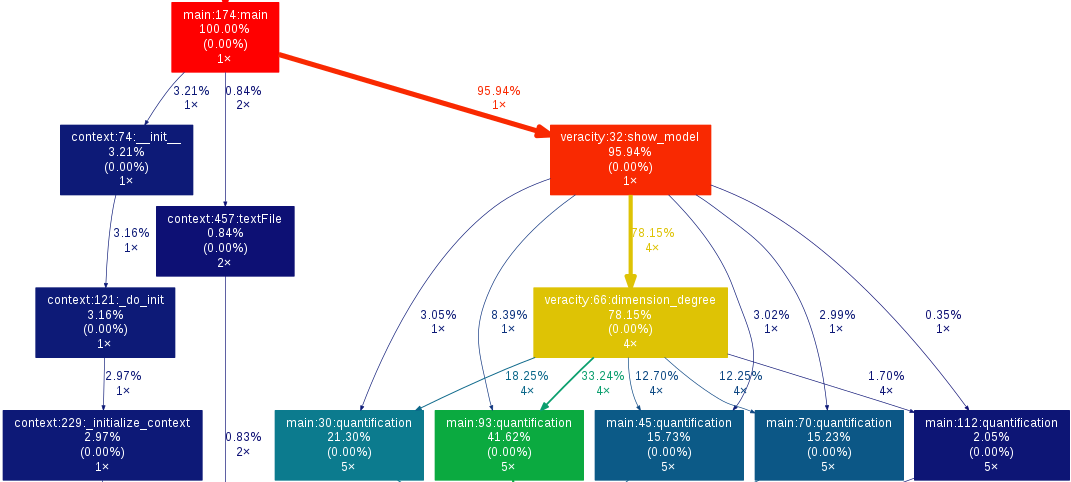
\includegraphics[scale=0.45]{max900.png}
\caption{doc5223.xml profiling 效能分析}
\label{max900}
\end{figure}

\begin{table}[H]
\caption{doc3.xml 計算效能}
\label{doc3pro}
\begin{center}
\begin{tabular}{|p{4cm}<{\centering}|p{3cm}<{\centering}|}
\hline
物件名稱 & 消耗效能 (\%)\\
\hline
document\_version & 32.49 \\
\hline
document\_encoding & 7.81 \\
\hline
document\_standalone & 6.82 \\
\hline
document\_valid & 14.26 \\
\hline
document\_depth & 12.17 \\
\hline
\end{tabular}
\end{center}
\end{table}

\begin{table}[H]
\caption{doc5223.xml 計算效能}
\label{doc5223pro}
\begin{center}
\begin{tabular}{|p{4cm}<{\centering}|p{3cm}<{\centering}|}
\hline
物件名稱 & 消耗效能 (\%)\\
\hline
document\_version & 21.30 \\
\hline
document\_encoding & 15.73 \\
\hline
document\_standalone & 15.23 \\
\hline
document\_valid & 41.62 \\
\hline
document\_depth & 2.05 \\
\hline
\end{tabular}
\end{center}
\end{table}

綜合上profiling的實驗結果可以觀察到,在處理大檔案的時候,document\_valid()的屬性會是效能瓶頸。而在處理小檔案的時候反而是document\_version()會是效能瓶頸,這兩個部分可以做效能上改善。
\newpage